\section{Method}
\label{sec:method}


\subsection{Problem Formulation}
\label{sec:method_formulation}

\noindent\textbf{AnyDepth-YOLO.}
We build on AnyDepth-YOLO~\cite{kang2026anydepth}, an object detector that enables multiple accuracy--efficiency operating points within a single model.
Each stage in both the backbone and the detection neck consists of an essential path that always executes and a skippable refinement path, allowing the detector to operate at different execution depths.
We consider two extreme configurations: a \emph{super} path, which executes both the shared essential path and all refinement paths (highest accuracy, highest computation cost), and a \emph{base} path, which executes only the shared essential path without any refinement (lowest computation cost with a modest accuracy drop).
% The detector is trained once and kept frozen, and at inference time the only decision is the selection of execution depth for each input frame under varying computation budgets.


\begin{figure*}[!ht]
\centering
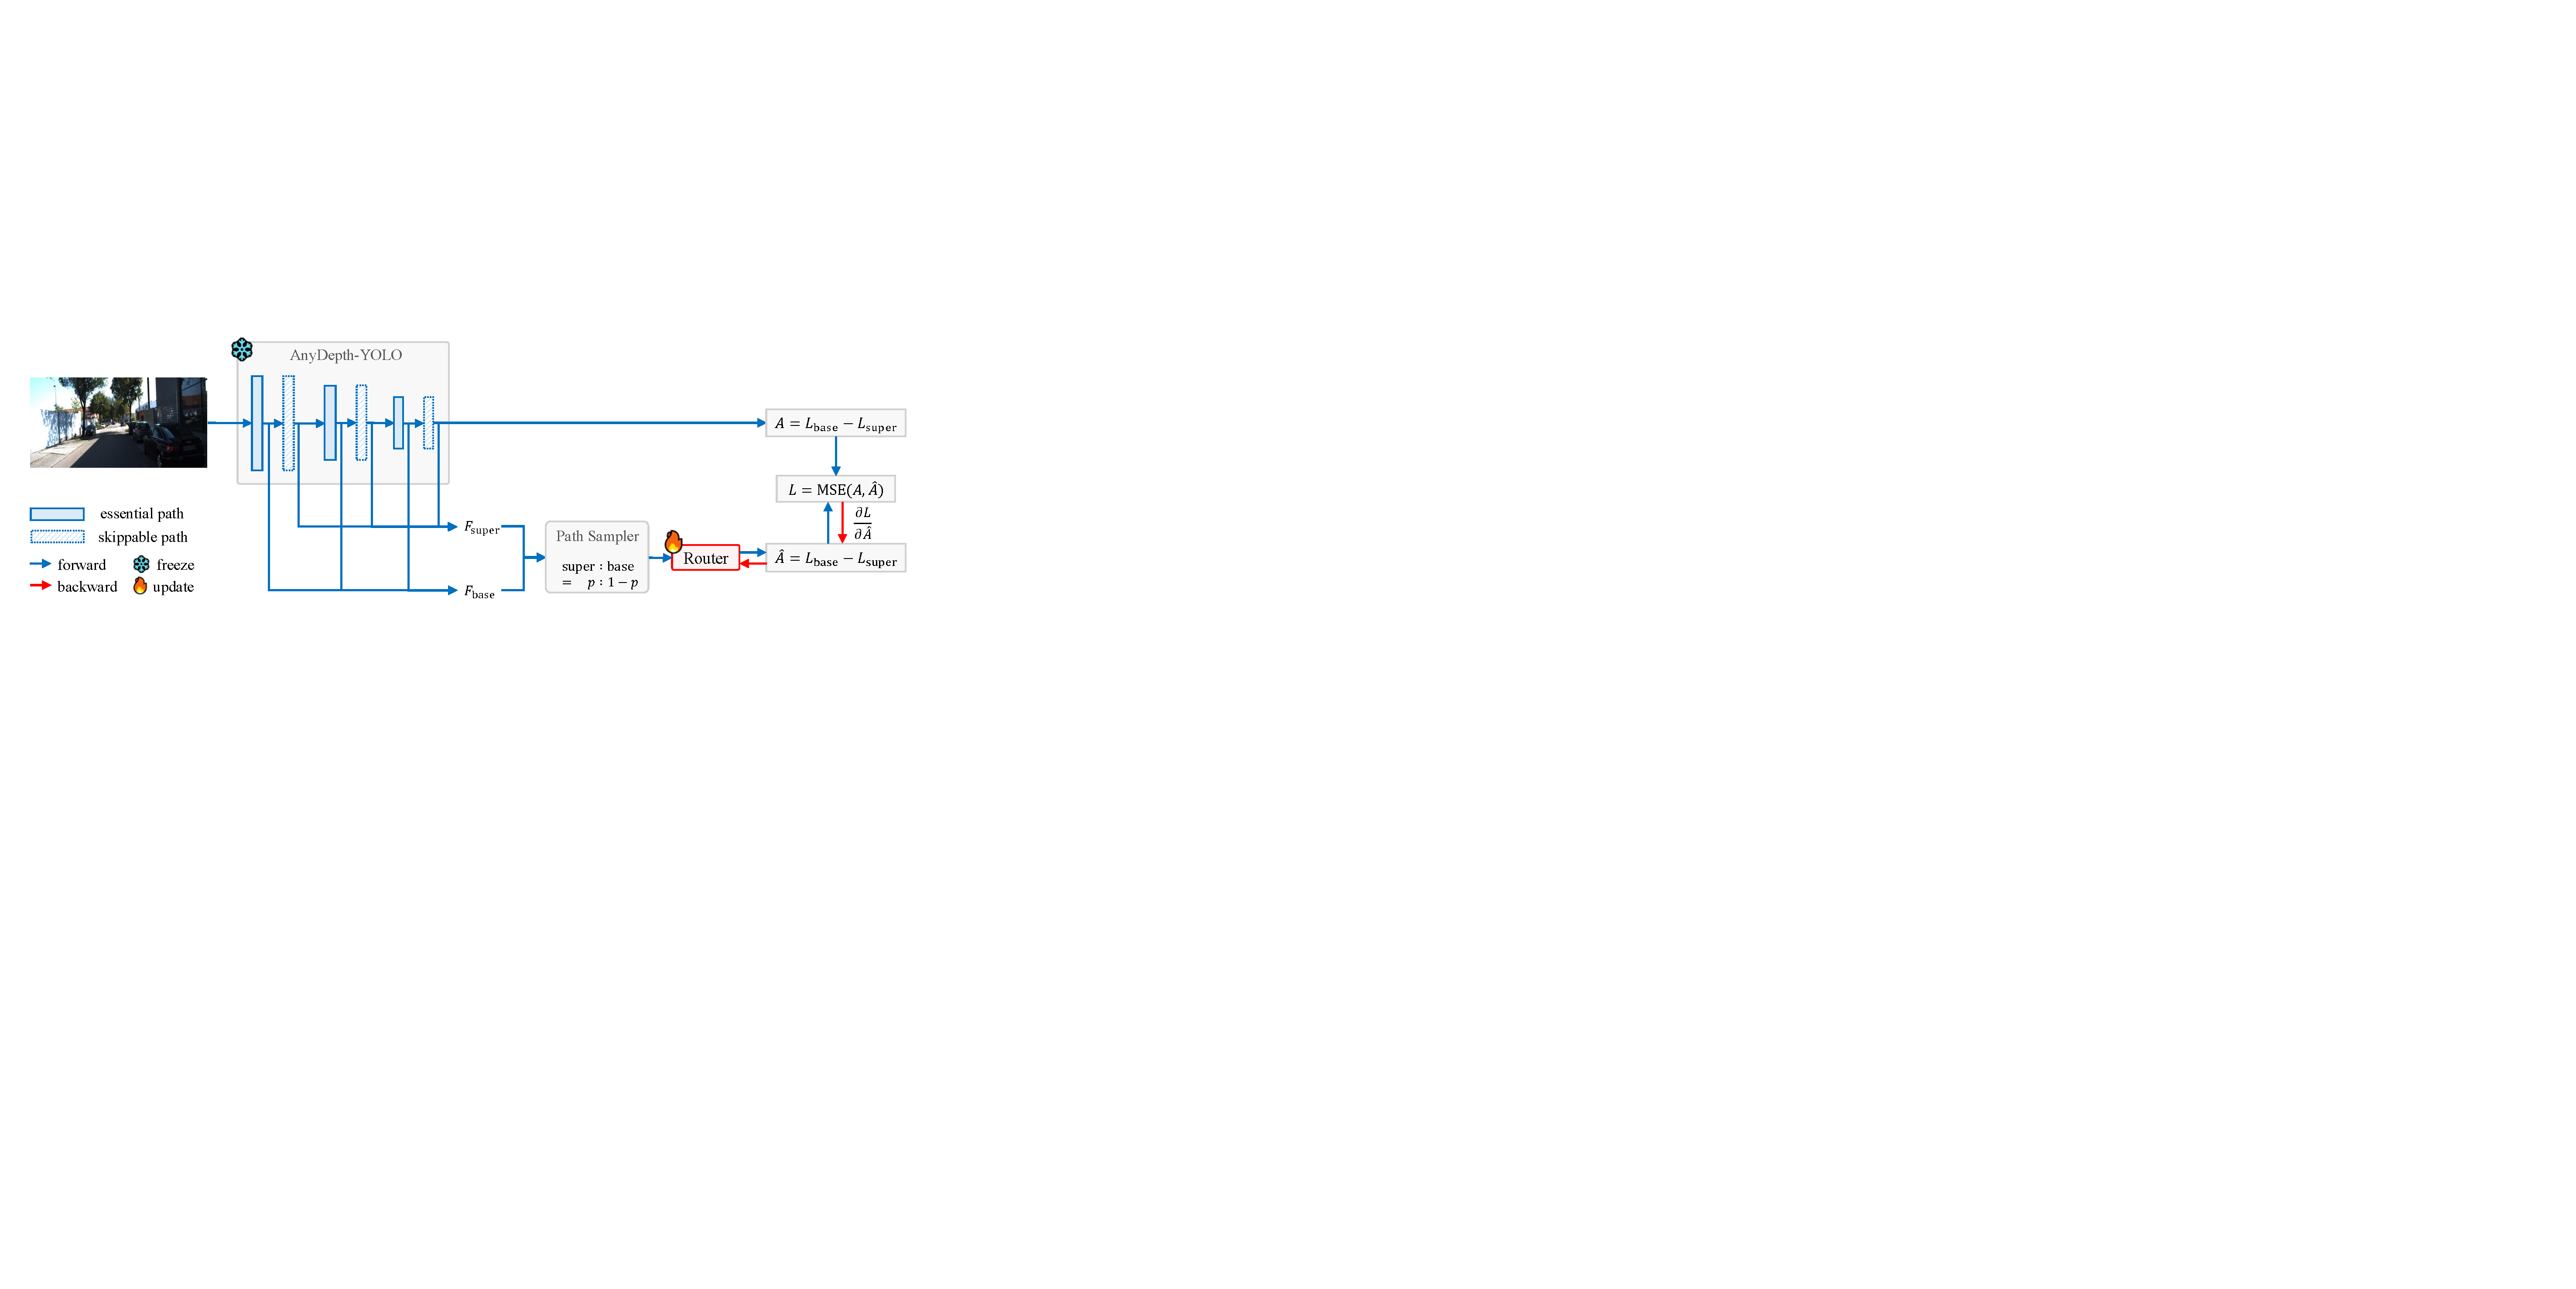
\includegraphics[width=0.85\textwidth]{fig_train.pdf}
\caption{
    Training pipeline. 
    The AnyDepth-YOLO detector is frozen; both paths are run once per image to obtain the true advantage $A=L_{\text{base}}-L_{\text{super}}$, and only the router is updated. 
    The router predicts $\hat{A}$ from the multi-scale intermediate features and is trained with $\text{MSE}(\hat{A},A)$ (blue: forward, red: backward).
}
\label{fig:train}
\end{figure*}

\begin{figure}[!ht]
\centering
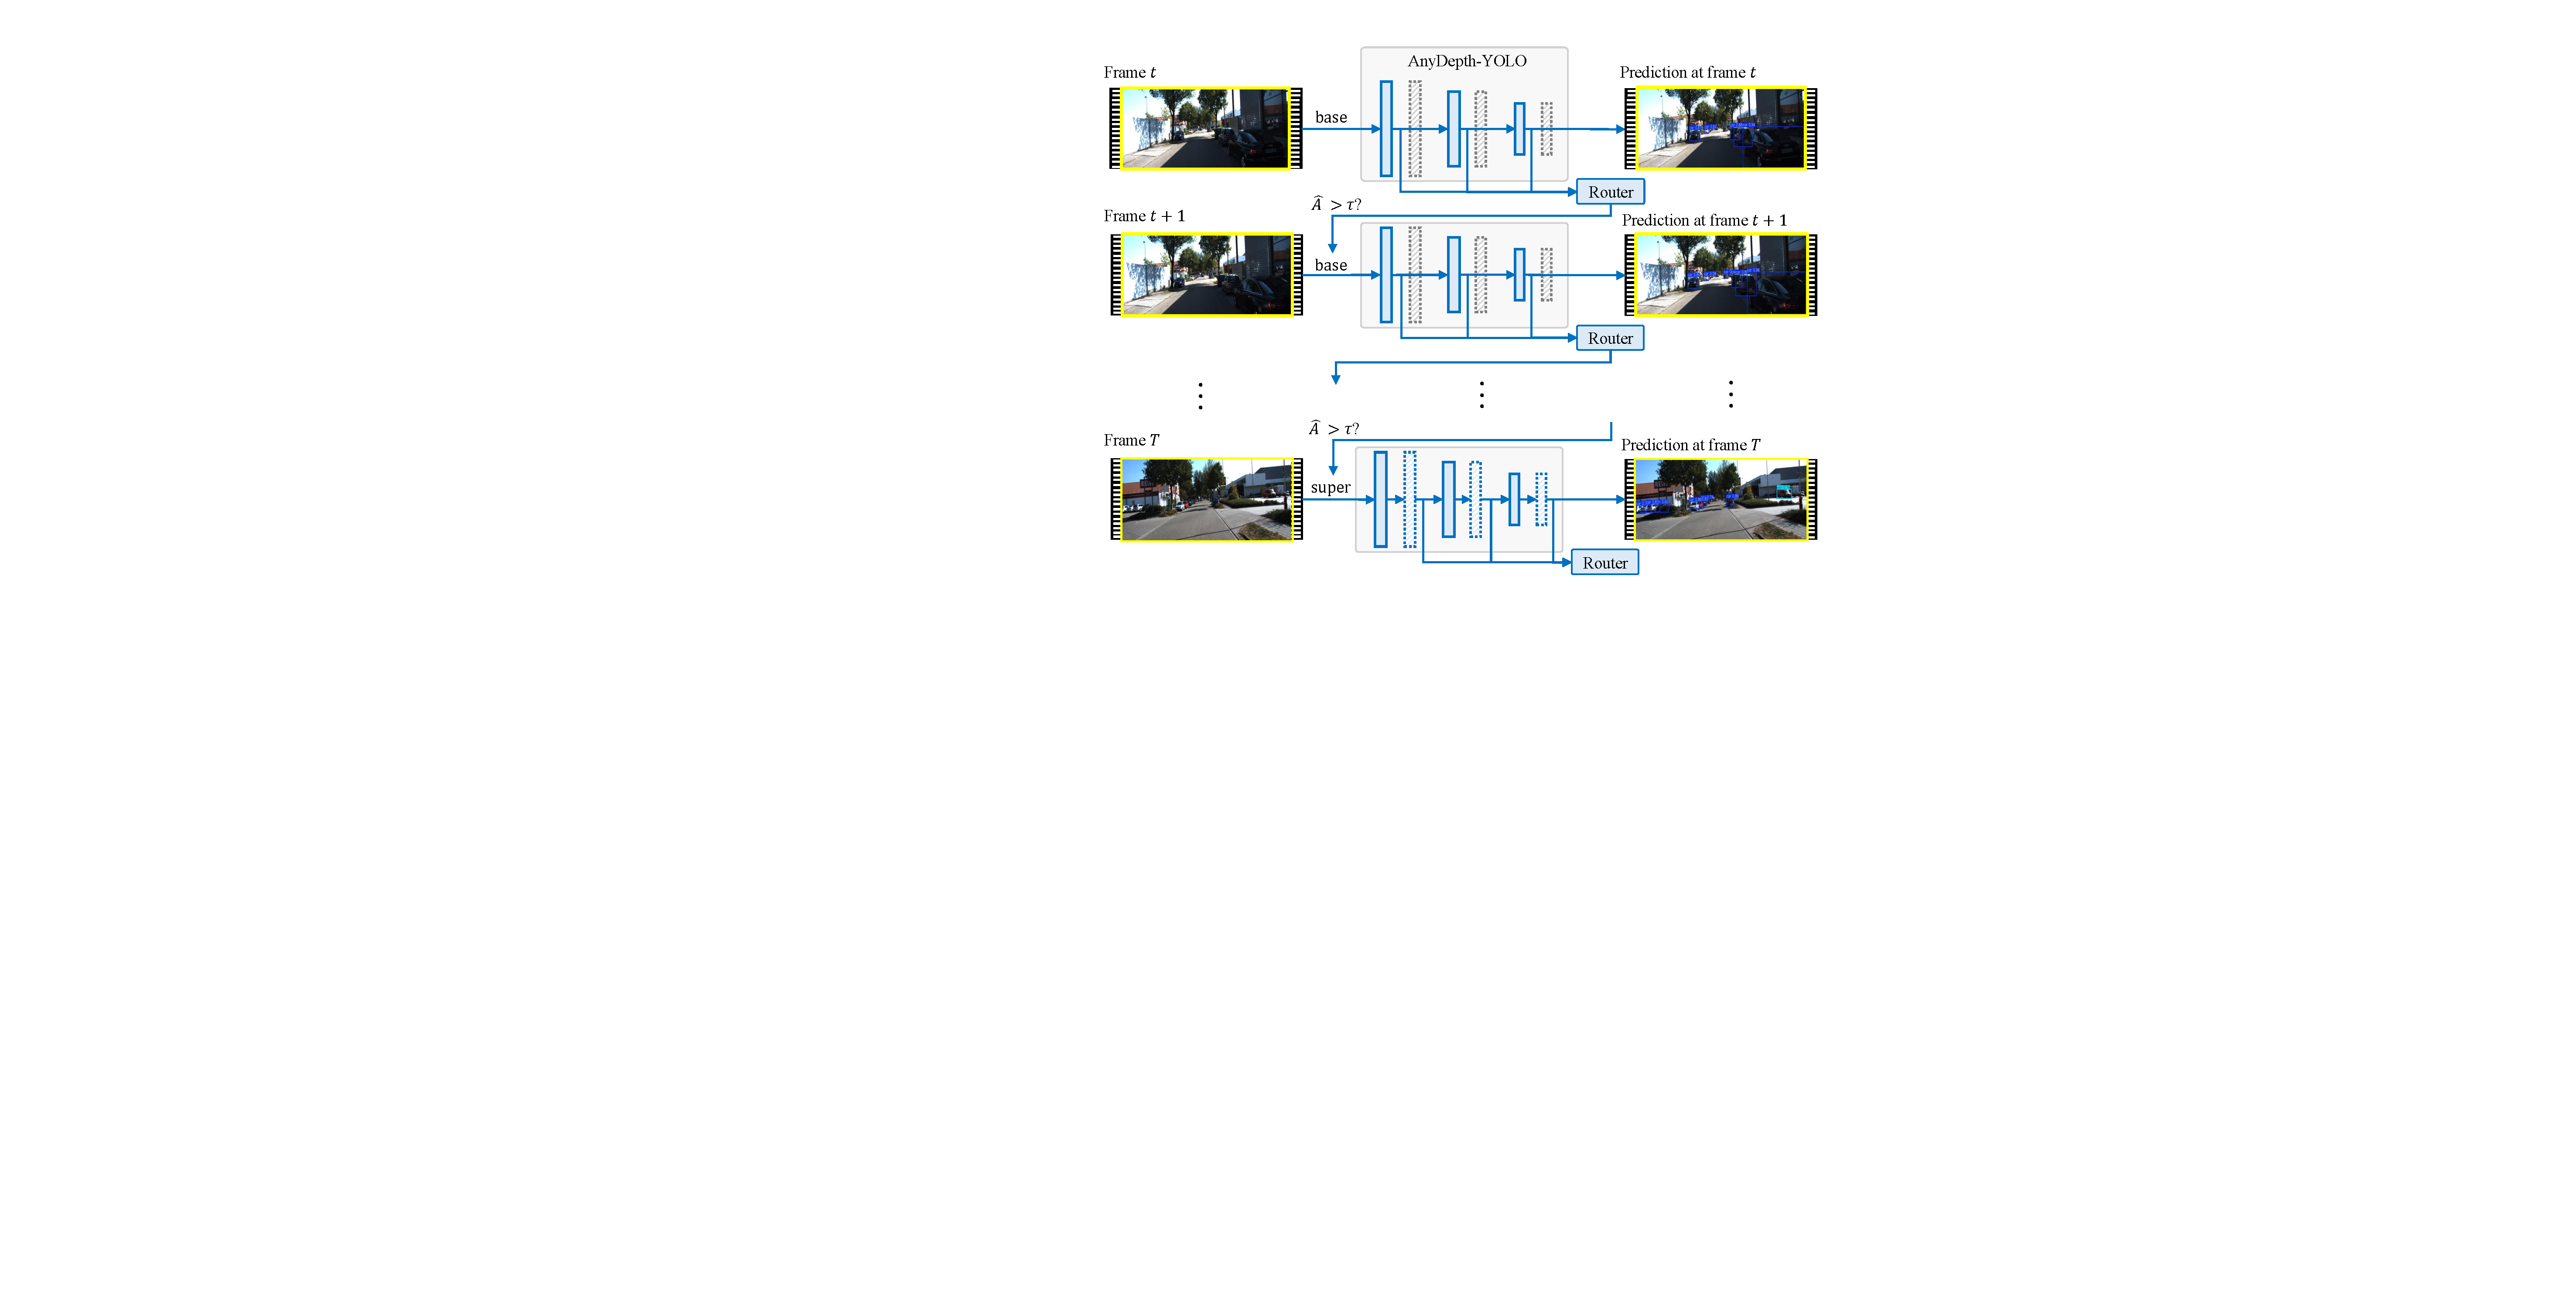
\includegraphics[width=0.5\textwidth]{fig_eval.pdf}
\caption{
    Causal routing mechanism for video streams.
    At each frame the detector runs the chosen path and the router predicts $\hat{A}$ from its intermediate features; the decision $\hat{A}>\tau$ selects the path (base or super) for the next frame. 
    Routing is causal and recursive across frames $t,t{+}1,\dots,T$, adding only the lightweight router forward.
}
\label{fig:eval}
\end{figure}


\medskip
\noindent\textbf{Routing problem.}
We thus formulate the decision space as a binary selection between two execution paths: a deep super configuration $\delta_{\text{}}$ and a shallow base configuration $\delta_{\text{base}}$. 
For each input image, we define the \emph{super advantage} as the reduction in detection loss obtained by using the deep path:
\begin{equation}
A = L_{\text{base}} - L_{\text{super}},
\label{eq:advantage}
\end{equation}
where $L_{\text{base}}$ and $L_{\text{super}}$ are the per-image detection
losses of the two paths. 
At deployment, the router exploits the strong temporal correlation between adjacent video frames, predicting an advantage score $\hat{A}$ from features generated on the previous frame and using a threshold $\tau$ to select the execution configuration for the current frame:
\begin{equation}
\text{config} =
\begin{cases}
\delta_{\text{super}}, & \hat{A} > \tau,\\[2pt]
\delta_{\text{base}},  & \text{otherwise.}
\end{cases}
\label{eq:route}
\end{equation}


\subsection{Router Training}
\label{sec:method_training}
Figure~\ref{fig:train} illustrates the conceptual training framework.
To ensure training efficiency, we run both execution paths once per training image offline to extract the multi-scale intermediate features (from the P3, P4, and P5 stages) along with their corresponding detection losses.
By precomputing and caching these values, the router can be trained extensively without the need for repeated detector forward passes.
Furthermore, because the underlying detector parameters remain strictly fixed, the true advantage $A$ serves as a stationary regression target throughout this process.


\begin{table}[t]
\caption{Router overhead (per frame, batch $1$). Every variant adds negligible cost
relative to the SUPER path ($26.30$ GFLOPs); the deployed router is TinyConv on both feature sources.}
\label{tab:overhead}
\centering
\begin{tabular}{llrrr}
\toprule
Router & Feature & \#Params & GFLOPs & \% of SUPER\\
\midrule
GAP-MLP & backbone & 60{,}241 & $1.17\times10^{-4}$ & $0.0004$\\
TinyConv & backbone & 60{,}881 & $4.17\times10^{-4}$ & $0.0015$\\
TinyConv & neck & 52{,}433 & $3.51\times10^{-4}$ & $0.0013$\\
TinyConv & both & 112{,}017 & $7.65\times10^{-4}$ & $0.0028$\\
\bottomrule
\end{tabular}
\end{table}


\medskip
\noindent\textbf{Router Architecture.}

The router predicts $\hat{A}$ from multi-scale features tapped from the frozen detector. 
Features can be extracted from the backbone, the detection neck, or their concatenation; we treat the feature source as a design choice and ablate it in Section~\ref{sec:abl_feature}, adopting the concatenation of both by default.
To keep routing overhead negligible, we explore two lightweight architectures. 
First, GAP-MLP discards spatial layout entirely by globally average-pooling each pyramid level and concatenating the resulting feature vectors. 
Second, TinyConv-MLP preserves coarse spatial context: multi-scale features are first adaptively pooled to a common $G\times G$ grid (default $2\times2$) and stacked along the channel dimension, after which a lightweight $3\times3$ depthwise convolution performs spatial mixing before global pooling. 
In both variants, the final merged representation is directly mapped to $\hat{A}$ by a two-layer fully connected head. 
As shown in Table~\ref{tab:overhead}, both designs introduce negligible computational overhead.



\medskip
\noindent\textbf{Training Objective.}
We train the router using a standard mean squared error (MSE) objective:
\begin{equation}
L_{\text{acc}} = \| A - \hat{A} \|^2.
\label{eq:loss}
\end{equation}
Crucially, unlike efficiency-aware routing objectives of the form
$\lambda_{\text{acc}}L_{\text{acc}} + \lambda_{\text{flops}}L_{\text{flops}}
(+\,\lambda_{\text{uni}}L_{\text{uni}})$, our objective contains no efficiency
weight $\lambda$ and no anti-collapse term. 
Consequently, the deployment operating point is not rigidly fixed during training, and the router simply learns to rank images based on how much the deep path improves detection.


\medskip
\noindent\textbf{Path-Conditioned Training.}
To ensure robust deployment, the router must remain well-calibrated to the feature distributions of both execution paths, as its input at test time depends entirely on whichever configuration was selected for the preceding frame. 
To prevent router training from favoring a single distribution, we simulate the prior frame's routing decision using a balanced action-sampling strategy. 
Specifically, for each training sample, we feed the router the features corresponding to the super path with probability $p$, and the base path features otherwise. 
This balanced exposure explicitly models the conditional execution loop of deployment, ensuring that the advantage predictor stays calibrated regardless of upstream routing choices.
The complete training procedure is summarized in Algorithm~\ref{alg:training}.



\begin{figure*}[!ht]
\centering
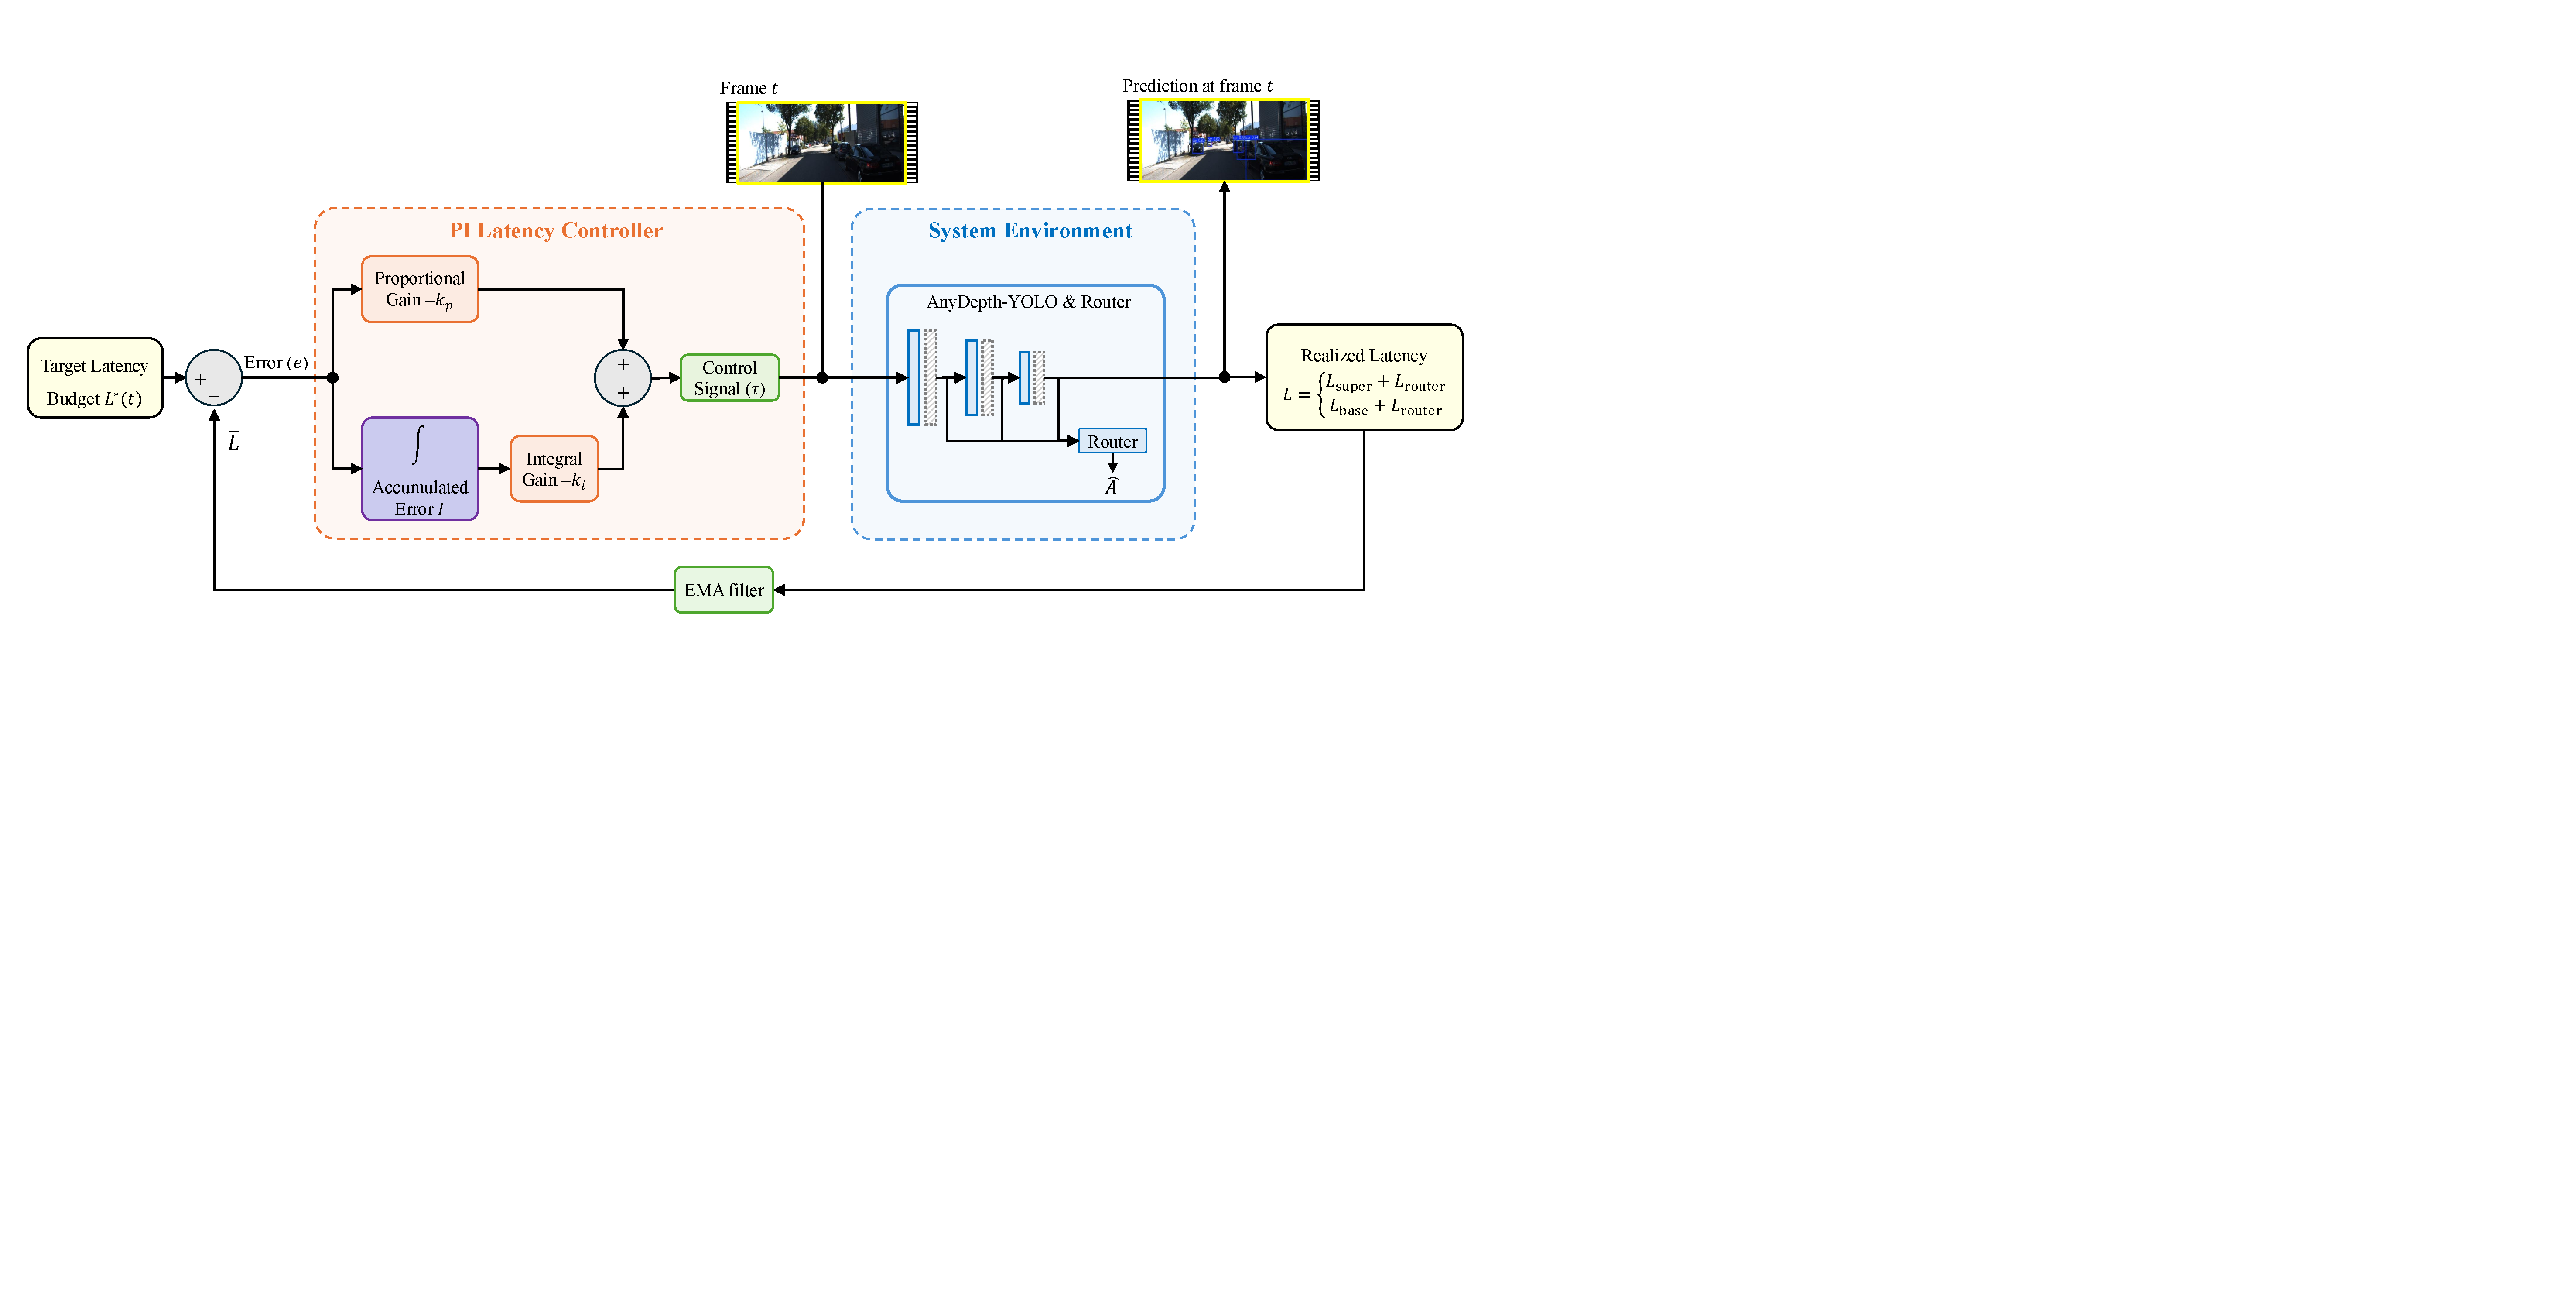
\includegraphics[width=0.95\textwidth]{fig_PI_controller.pdf}
\caption{PI control of the routing threshold $\tau$. The error between the latency
budget $L^\star(t)$ and an EMA $\bar{L}$ of the realized per-frame latency is fed
through proportional ($k_p$) and integral ($k_i$) terms that nudge $\tau$; a lower
$\tau$ sends more frames to the super path (higher latency) and vice versa,
closing the loop so the realized latency tracks the budget.}
\label{fig:pi_controller}
\end{figure*}


\subsection{Router Deployment}
\label{sec:method_deploy}

Once trained, the router operates as a causal, per-frame controller whose inference-time behavior is entirely governed by the routing threshold $\tau$. 
To validate its practical utility, we evaluate the router under two distinct deployment paradigms based on how $\tau$ is managed: serving static operating points for standardized benchmarking, and dynamically tracking a latency budget for real-world application.

\textbf{Threshold-Based Routing for Benchmarking.}
Because the router is trained solely to predict the expected loss reduction, the deployment operating point is fully decoupled from the training phase. 
The threshold $\tau$ in Equation~\eqref{eq:route} acts as a free dial: raising $\tau$ routes fewer images to the deep path (saving compute at the cost of accuracy), while lowering it does the opposite. 
Consequently, sweeping $\tau$ systematically shifts the dataset-averaged accuracy and computational cost, tracing a continuous accuracy--efficiency Pareto curve from a single trained model.
For continuous video streams, routing is strictly causal (Figure~\ref{fig:eval}). To prevent the router from introducing a latency bottleneck, the path decision for frame $t+1$ is made using the intermediate features already generated by the path executed on frame $t$. 
Exploiting the temporal continuity of video data, this allows the router to commit to a path at the start of each frame without requiring an extra detector forward pass. 

\textbf{Online Latency-Budget Control for Real-World Deployment.}
While a fixed $\tau$ maintains a static operating point, real-world edge devices frequently face time-varying compute constraints (e.g., due to thermal throttling or battery limits). 
Thanks to the single-scalar nature of $\tau$, the system can dynamically adapt to a shifting latency budget $L^\star(t)$ online without any retraining. 
As illustrated in Figure~\ref{fig:pi_controller}, we wrap the routing loop in a standard proportional--integral (PI) controller. 
The controller maintains an exponential moving average (EMA) $\bar{L}$ of the realized per-frame latency. 
It computes the error $e = L^\star(t) - \bar{L}$ and incrementally adjusts $\tau$ by $-k_p e - k_i I$ (where $I$ is the accumulated integral error). 
Because lowering $\tau$ routes more frames to the super path (thereby increasing latency) and raising $\tau$ has the inverse effect, this closed-loop mechanism continuously nudges the realized latency to track the target budget. 
This threshold-based loop is summarized in Algorithm~\ref{alg:routing}.

\begin{algorithm}[!t]
\caption{Causal budget-adaptive depth routing (deployment)}
\label{alg:routing}
\small
\begin{tabular}{@{}r@{\hspace{5pt}}p{0.90\columnwidth}@{}}
\multicolumn{2}{@{}p{0.95\columnwidth}@{}}{\textbf{Input:} frozen AnyDepth detector $D$, router $R$, target latency sequence $L^\star(t)$,}\\
\multicolumn{2}{@{}p{0.95\columnwidth}@{}}{\hphantom{\textbf{Input:} }PI gains $k_p, k_i$, EMA momentum $\alpha$, frames $x_1,\dots,x_T$}\\
\multicolumn{2}{@{}p{0.95\columnwidth}@{}}{\textbf{Output:} streaming per-frame detections $y_t$}\\[2pt]
$1$ & $\mathit{config} \leftarrow \delta_{\text{base}}$ \hfill{\footnotesize\itshape $\triangleright$ initialize with base configuration}\\
$2$ & $\tau \leftarrow \tau_0, \;\bar{L} \leftarrow L^\star(1), \;I \leftarrow 0$ \hfill{\footnotesize\itshape $\triangleright$ initialize PI controller state}\\
$3$ & \textbf{for} $t=1$ \textbf{to} $T$ \textbf{do}$:$\\
$4$ & \quad $(y_t, f_t) \leftarrow D(x_t, \mathit{config})$ \hfill{\footnotesize\itshape $\triangleright$ execute chosen configuration}\\
$5$ & \quad $\hat{A} \leftarrow R(f_t)$ \hfill{\footnotesize\itshape $\triangleright$ predict advantage for next frame}\\
$6$ & \quad $\mathit{config} \leftarrow \delta_{\text{super}}$ \textbf{if} $\hat{A} > \tau$ \textbf{else} $\delta_{\text{base}}$ \hfill{\footnotesize\itshape $\triangleright$ route $x_{t+1}$}\\
$7$ & \quad $l_t \leftarrow \text{MeasureLatency}()$ \hfill{\footnotesize\itshape $\triangleright$ observe realized per-frame latency}\\
$8$ & \quad $\bar{L} \leftarrow (1-\alpha)\bar{L} + \alpha l_t$ \hfill{\footnotesize\itshape $\triangleright$ update EMA of latency}\\
$9$ & \quad $e \leftarrow L^\star(t) - \bar{L}$ \hfill{\footnotesize\itshape $\triangleright$ compute latency tracking error}\\
$10$& \quad $I \leftarrow I + e$ \hfill{\footnotesize\itshape $\triangleright$ accumulate integral error}\\
$11$& \quad $\tau \leftarrow \tau - k_p e - k_i I$ \hfill{\footnotesize\itshape $\triangleright$ adjust threshold dynamically}\\
$12$& \quad \textbf{emit} $y_t$ \hfill{\footnotesize\itshape $\triangleright$ stream detection output}\\
$13$& \textbf{end for}
\end{tabular}
\end{algorithm}



% Temp ---------


% \begin{algorithm}[!t]
% \caption{Path-conditioned router training}
% \label{alg:training}
% \small
% \begin{tabular}{@{}r@{\hspace{5pt}}p{0.90\columnwidth}@{}}
% \multicolumn{2}{@{}p{0.95\columnwidth}@{}}{\textbf{Input:} cached dataset $\mathcal{X}$ (containing features $F$ and losses $L$), router $R$, sampling ratio $p$, learning rate $\eta$}\\
% \multicolumn{2}{@{}p{0.95\columnwidth}@{}}{\textbf{Output:} optimized router parameters $\theta$}\\[2pt]
% $1$ & \textbf{for} each training step \textbf{do}$:$\\
% $2$ & \quad Sample mini-batch $\mathcal{B} \subset \mathcal{X}$\\
% $3$ & \quad $A \leftarrow L_{\mathcal{B}}^{\text{base}} - L_{\mathcal{B}}^{\text{super}}$ \hfill{\footnotesize\itshape $\triangleright$ ground-truth advantage vector}\\
% $4$ & \quad $\mathit{config} \sim \text{Sample}(\{\delta_{\text{super}}, \delta_{\text{base}}\}, p)$ \hfill{\footnotesize\itshape $\triangleright$ path-conditioned sampling}\\
% $5$ & \quad $\hat{A} \leftarrow R_\theta(F_{\mathcal{B}}^{\mathit{config}})$ \hfill{\footnotesize\itshape $\triangleright$ batch forward pass on selected features}\\
% $6$ & \quad $\theta \leftarrow \theta - \eta \nabla_\theta \| A - \hat{A} \|^2$ \hfill{\footnotesize\itshape $\triangleright$ update router parameters}\\
% $7$ & \textbf{end for}
% \end{tabular}
% \end{algorithm}